\documentclass[11pt]{article}
\usepackage{amssymb}
\usepackage{amsthm}
\usepackage{enumitem}
\usepackage{physics,amsmath}
\usepackage{bm}
\usepackage{adjustbox}
\usepackage{mathrsfs}
\usepackage{graphicx}
\usepackage{siunitx}
\usepackage[mathscr]{euscript}

\title{\textbf{Solved selected problems of Classical Mechanics - Gregory}}
\author{Franco Zacco}
\date{}

\addtolength{\topmargin}{-3cm}
\addtolength{\textheight}{3cm}

\newcommand{\hatr}{\bm{\hat{r}}}
\newcommand{\hatx}{\bm{\hat{x}}}
\newcommand{\haty}{\bm{\hat{y}}}
\newcommand{\hatz}{\bm{\hat{z}}}
\newcommand{\hatth}{\bm{\hat{\theta}}}
\newcommand{\hatphi}{\bm{\hat{\phi}}}
\newcommand{\hatrho}{\bm{\hat{\rho}}}
\theoremstyle{definition}
\newtheorem*{solution*}{Solution}
\renewcommand*{\proofname}{Solution}

\begin{document}
\maketitle
\thispagestyle{empty}

\section*{Chapter 8 - Non-linear oscillations and phase space}

	\begin{proof}{\textbf{8.2}}
        Let us define $s = \omega(\epsilon) t$ and change variables so
        the equation is written in terms of $s$ then
        \begin{align*}
            (\omega(\epsilon))^2 x'' + x + \epsilon x^5 = 0
        \end{align*}
        By Lindstedt's method, we know there is a solution to this equation
        in the form of the perturbation series
        $$x(s,\epsilon) = x_0(s) + \epsilon x_1(s) + \epsilon^2 x_2(s) + ...$$
        and the same for $\omega(\epsilon)$ which is also part of the solution
        $$\omega(\epsilon) = 1 + \epsilon\omega_1 + \epsilon^2\omega_2 + ...$$
        So by replacing these we get that
        \begin{align*}
            (1 + \epsilon\omega_1 + &\epsilon^2\omega_2 + ...)^2
            (x_0'' + \epsilon x_1'' + \epsilon^2 x_2'' + ...) +\\
            &(x_0 + \epsilon x_1 + \epsilon^2 x_2 + ...) +
            \epsilon(x_0 + \epsilon x_1 + \epsilon^2 x_2 + ...)^5 = 0
        \end{align*}
        Now we can equate coefficients of powers of $\epsilon$ so
        we get a succession of ODEs and initial contitions, the first two of
        which are as follows
        $$x_0'' + x_0 = 0\quad\quad (\text{zero-order})$$
        With $x_0 = 1$ and $x_0' = 0$ when $s = 0$ also we have
        $$x_1'' + x_1 = -2\omega x_0'' - x_0^5 \quad\quad (\text{first-order})$$
        With $x_1 = 0$ and $x_1' = 0$ when $s = 0$. The solution to the
        zero-order equation is
        $$x_0(s) = \cos(s)$$
        And we can substitute this in the first-order equation as follows
        \begin{align*}
            x_1'' + x_1 &= 2\omega_1 \cos(s) - \cos^5(s)\\
            x_1'' + x_1 &= \frac{1}{8}(16\omega_1 - 5)\cos(s) - \frac{5}{16}\cos(3s) - \frac{1}{16}\cos(5s)
        \end{align*}
        Where we used the identity $16\cos^5(s) = 10\cos(s) + 5\cos(3s) + \cos(5s)$.
        Also, we see that the first term of the right-hand side must be 0
        otherwise $x_1(s)$ wouldn't be periodic then
        $$\omega_1 = \frac{5}{16}$$
        This equation can now be solved by standard methods and we get that
        \begin{align*}
            x_1(s) = A\sin(s) + B\cos(s) + \frac{5}{128}\cos(3s) + \frac{1}{384}\cos(5s)
        \end{align*}
        Now by replacing with the initial conditions we get that the constant
        $B$ is
        \begin{align*}
            0 &=  B + \frac{5}{128} + \frac{1}{384}\\
            B &= -\frac{1}{24}
        \end{align*}
        And computing $x_1'(s)$ we can get the constant $A$ as
        \begin{align*}
            x_1'(s) &= A\cos(s) - B\sin(s) -\frac{15}{128}\sin(3s) -\frac{5}{384}\sin(5s) \\
            0 &= A\cos(0) - B\sin(0) -\frac{15}{128}\sin(0) -\frac{5}{384}\sin(0) \\
            A &= 0
        \end{align*}
        The solution to the first-order equation is then
        \begin{align*}
            x_1(s) = -\frac{1}{24}\cos(s) + \frac{5}{128}\cos(3s) + \frac{1}{384}\cos(5s)
        \end{align*}
        Finally, we have that when $\epsilon$ is small then
        $$\omega(\epsilon) = 1 + \frac{5}{16}\epsilon + O(\epsilon^2)$$
        and
        \begin{align*}
            x(s) = \cos(s) + \epsilon\left(-\frac{1}{24}\cos(s) +
            \frac{5}{128}\cos(3s) + \frac{1}{384}\cos(5s)\right) + O(\epsilon^2)
        \end{align*}
        where $s = (1 + \frac{5}{16}\epsilon + O(\epsilon^2))t$.
    \end{proof}
\cleardoublepage
	\begin{proof}{\textbf{8.5}}
        Let
        \begin{align*}
            \dot{x_1} = F_1(x_1,x_2,t) \quad\quad \dot{x_2} = F_2(x_1,x_2,t)
        \end{align*}
        Also, we know that $r = \sqrt{x_1^2 + x_2^2}$ then
        \begin{align*}
            \dot{r} &= \frac{x_1\dot{x_1} + x_2\dot{x_2}}{\sqrt{x_1^2 + x_2^2}}\\
            \dot{r} &= \frac{x_1F_1 + x_2F_2}{r}
        \end{align*}
        On the other hand, we know that $\tan\theta = \sin\theta/\cos\theta$ then
        \begin{align*}
            \tan\theta &= \frac{r\sin\theta}{r\cos\theta}\\
            \theta &= \tan^{-1}\frac{x_2}{x_1}
        \end{align*}
        And the derivative of $\theta$ is
        \begin{align*}
            \dot{\theta} &= \frac{x_1\dot{x_2} - x_2\dot{x_1}}{x_1^2 + x_2^2}\\
            \dot{\theta} &= \frac{x_1F_2 - x_2F_1}{r^2}
        \end{align*}

        Now let us convert the following system to the polar form
        \begin{align*}
            \dot{x} &= -x+y\\
            \dot{y} &= -x-y
        \end{align*}
        Then by using the equations we just derived we have that
        \begin{align*}
            \dot{r} &= \frac{x(-x+y) + y(-x-y)}{r}\\
            \dot{r} &= \frac{-(x^2+y^2)}{r} = \frac{-r^2}{r} = -r
        \end{align*}
        and
        \begin{align*}
            \dot{\theta} &= \frac{x(-x-y) - y(-x+y)}{r^2}\\
            \dot{\theta} &= \frac{-x^2-y^2}{r} = \frac{-r^2}{r^2} = -1
        \end{align*}
        So we have two ODEs that we can solve with standard methods to obtain
        $$r = Ae^{-t} \quad\quad \theta = -t + B$$
        As $t$ goes to infinity we see  that $\theta$ tends to $-\infty$ and $r$
        tends to $0$ so the phase path must encircle the origin and end up there
        no matter which are the initial conditions. Also, the phase paths
        rotate clockwise because the negative sign we see for $\dot{\theta}$.
    \end{proof}
\cleardoublepage
    \begin{proof}{\textbf{8.7}}
        From the damped oscillator equation
        $$\ddot{x} + \dot{x} + x = 0$$
        we can get two first-order ODEs by replacing variables as follows
        \begin{align*}
            \dot{x} &= y\\
            \dot{y} &= -y - x
        \end{align*}
        Now we can derive the polar equations by replacing values in the
        equations we determined in problem 5. We also use that $x = r\cos\theta$
        and $y= r\sin\theta$ then
        \begin{align*}
            \dot{r} &= \frac{xy + y(-y-x)}{r} = \frac{-y^2}{r}\\
            \dot{r} &= -\frac{r^2\sin^2\theta}{r} = -r\sin^2\theta
        \end{align*}
        On the other hand for $\theta$ we get that
        \begin{align*}
            \dot{\theta} &= \frac{x(-y-x) - y^2}{r^2} = -\frac{x^2 +xy+ y^2}{r^2}\\
            \dot{\theta} &= -\frac{r^2+xy}{r^2} = -(1 + \cos\theta\sin\theta)\\
            \dot{\theta} &= -\left(1 + \frac{1}{2}\sin2\theta\right)
        \end{align*} 
        Now we want to check that the phase paths encircle the origin
        infinitely many times clockwise, i.e. we want to show that
        $\theta \to -\infty$ and $r \to 0$ when $t \to \infty$. From the
        equation of $\dot{\theta}$ we see that $\dot{\theta} \leq -1/2$ then
        this implies that
        \begin{align*}
            \theta &\leq -1/2t + A
        \end{align*}
        So when $t \to \infty$ we have that $\theta \to -\infty$ no matter the
        initial conditions i.e. the phase paths encircle the origin clockwise.
        
        Finally, let us check that $r \to 0$ when $t \to \infty$ by solving the
        equation. So we see that
        \begin{align*}
            \int \frac{dr}{r} &= - \int \sin^2\theta~dt\\
            -\log(r) &= \int \sin^2\theta~dt\\
            -\log(r) &= \int \frac{\sin^2\theta}{\dot\theta}~d\theta
        \end{align*}
        Since $\dot\theta \leq -1/2$ then we can do the following analysis
        \begin{align*}
            -\log(r) &= \int \frac{\sin^2\theta}{\dot\theta}~d\theta\\
                &\geq -2\int \sin^2\theta~d\theta\\
                &= \frac{1}{2}\sin(2\theta) - \theta + C
        \end{align*}
        Since when $t \to \infty$ then $\theta \to -\infty$ we see that 
        $\frac{1}{2}\sin(2\theta) - \theta + C \to \infty$ no matter the initial
        conditions (i.e. the value of $C$). Therefore $-\log(r) \to \infty$ when
        $t \to \infty$ then $r \to 0$.
    \end{proof}
\cleardoublepage
    \begin{proof}{\textbf{8.10}}
        Consider the symmetrical predator-prey equations
        \begin{align*}
            \dot{x} &= x - xy\\
            \dot{y} &= xy - y
        \end{align*}
        We want to determine the phase path equation so we write the path
        gradient as follows
        \begin{align*}
            \frac{dx}{dy} &= \frac{x - xy}{xy - y}\\
                &= \frac{x(1-y)}{y(x-1)}
        \end{align*}
        This is a separable ODE so we can solve it
        \begin{align*}
            \int \frac{x-1}{x}~dx &= \int \frac{1-y}{y}~dy\\
            x - \log(x) &= \log(y) - y + B\\
            e^{x - \log(x)} &= e^{\log(y) - y + B}\\
            x^{-1}e^x &= e^Bye^{-y}\\
            A &= (ye^{-y})(xe^{-x})
        \end{align*}
        Where we named $A = 1/e^B$.
        Let us now consider the equation $z = (ye^{-y})(xe^{-x})$ and let us
        plot it using a computer program. We get the following plot
        \begin{center}
            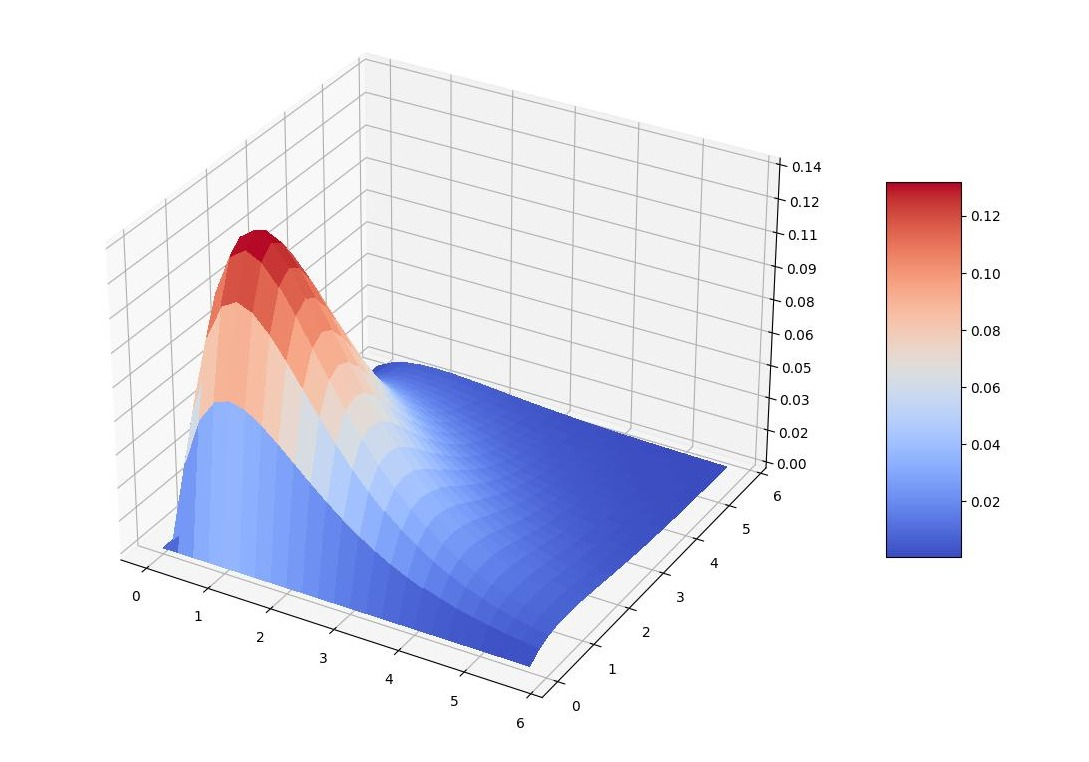
\includegraphics[scale=0.3]{ch8-10.jpg}
        \end{center}
        Where we see that if we intersect the plot with a horizontal plane,
        we get a closed curve that encircles the equilibrium point (1,1) as
        we wanted. 
    \end{proof}
\end{document}






















